\documentclass[12pt]{scrartcl}

% packages
\usepackage[
    a4paper, total={18cm, 26cm},
    left=0.75in,
    right=0.75in,
    top=0.75in,
    bottom=0.50in,
    footskip=15pt
]{geometry}
\usepackage{lastpage}
\usepackage{graphicx} % \includegraphics
\usepackage{amsmath} % math
\usepackage{fancyhdr} % header and footer
\usepackage[portuguese]{babel}
\usepackage{tabularx}
\usepackage{listings}
\usepackage{esdiff}

% configs
\setlength{\parindent}{0pt}

% comandos
\renewcommand{\familydefault}{\sfdefault}
\newcommand{\un}[1]{\;\textrm{#1}}
\newcommand{\logo}{\quad \Rightarrow \quad}
\newcommand{\fase}[1]{\ensuremath{\phase{{#1}^{\circ}}}}
\newcommand{\code}[1]{\texttt{#1}}

\graphicspath{ {./images/} }

\begin{document}

\lstset{frame=none,
  language=R,
  aboveskip=3mm,
  belowskip=3mm,
  showstringspaces=false,
  columns=flexible,
  basicstyle={\small\ttfamily},
  numbers=none,
  breaklines=true,
  breakatwhitespace=true,
  tabsize=4,
  extendedchars=true,
  literate={ç}{ã}{â}{é}{ê}1,
}


\numberwithin{figure}{section}
\numberwithin{equation}{section}
\numberwithin{table}{section}

\pagestyle{fancy}

\fancyhead{}
\fancyhead[L]{Estudo Dirigido 5}
\fancyhead[R]{EMA255 - Termodinâmica Computacional}
\fancyfoot{}
\fancyfoot[R]{Pág. \thepage \; / \pageref{LastPage}}

\begin{center}
    Aluno: Raphael Henrique Braga Leivas \\
    Matrícula: 2020028101 \\
    Professor Responsável: Márcio Ziviani \\[20pt]

    Código fonte LaTeX desse arquivo pode ser visto em meu GitHub pessoal: https://github.com/RaphaelLeivas/latex/tree/main/TermoComp
\end{center}

\hrule

\section{Questão 1}

O diagrama esquemático do problema está exibido na Figura \ref{fig:problemaplaca}.

\begin{figure}[h!]
    \caption{Diagrama do problema a ser analisado.}
    \label{fig:problemaplaca}
    \centering
    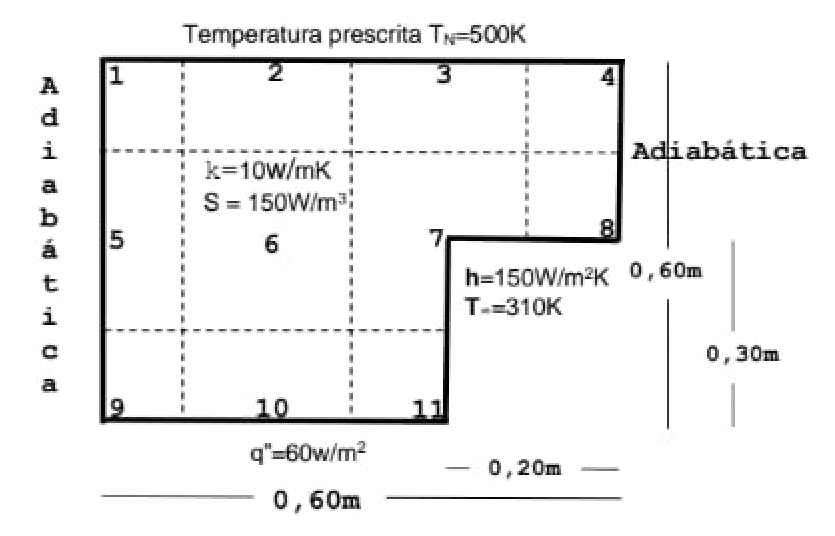
\includegraphics[scale=0.60]{problemaED05.png}
\end{figure}

Em regime permanente, o processo de condução na Figura \ref{fig:problemaplaca} possui 
equação dada por 

\begin{equation}\label{eq:pdecomplete}
    \frac{\partial}{\partial{x}} \left(k\frac{\partial{T}}{\partial{x}}\right) +
    \frac{\partial}{\partial{y}} \left(k\frac{\partial{T}}{\partial{y}}\right) +
    S = 0
\end{equation}

Em que o domínio de solução da equação diferencial parcial de \eqref{eq:pdecomplete} é

\begin{equation}\label{eq:domain}
    0 < x < 0,6 \un{m} \quad , \quad 0 < y < 0,6 \un{m}
\end{equation}

E as condições de contorno são:

\begin{itemize}
    \item Fronteira oeste: como é adiabática, temos $\diff{T}{x} = 0$;
    \item Fronteira norte: como temos tempeartura prescrita, temos $T(y=0,6) = 500 \un{K}$ ;
    \item Fronteira sul: como temos fluxo prescrito, temos, pela Lei de Fourier, $-k\diff{T}{y} = 60 \un{W/m$^2$}$
    \item Fronteira leste, parte inferior $x = 0,4 \un{m}$ e $0 < y < 0,3 \un{m}$, temos conveccção: $-k\diff{T}{x} = h\left(T(x=0,4) - T_{\infty}\right)$;
    \item Fronteira leste, parte superior $x = 0,6 \un{m}$ e $0,3 < y < 0,6 \un{m}$, temos adiabática: $\diff{T}{x} = 0$;
    \item Fronteira leste, parte deitada $y = 0,3 \un{m}$ e $0,4 < x < 0,6 \un{m}$, temos conveccção: $-k\diff{T}{y} = h\left(T(y=0,3) - T_{\infty}\right)$;
\end{itemize}

\section{Questão 2}

Para cada nó exibido na Figura \ref*{fig:problemaplaca}, aplicamos o balanço de energia para obter as equações de 
diferenças finitas de cada nó de 1 a 11 da malha. As expressões de cada nó foram retirada
da página 218 do livro do Incropera, sexta edição

\[  No 1: T_5 + T_2 + 2\frac{h \Delta x}{k} T_{\infty} - 2\left(\frac{h \Delta x}{k} + 1\right) T_1 = 0 \]
\[  No 1: T_5 + T_2 - 6,5 T_1 = -1395 \]

\[  No 2: T_1 + T_6 + T_3 - 3T_2 + 500 = 0 \]
\[  No 2: T_1 + T_6 + T_3 - 3T_2 = - 500 \]

\[  NO 3: T_2 + T_7 + T_4 - 3T_3 + 500 = 0 \]
\[  NO 3: T_2 + T_7 + T_4 - 3T_3 = - 500 \]

\[  NO 3: T_2 + T_7 + T_4 - 3T_3 + 500 = 0 \]
\[  NO 3: T_2 + T_7 + T_4 - 3T_3 = - 500 \]

\[  No 4: T_3 + T_8 - 6,5 T_4 = -1395 \]

\[  No 5: T_1 + T_6 + T_9 - 3T_5 = 0 \]

\[  No 6: T_2 + T_7 + T_5 - T_{10} - 4T_6 = 0 \]

% \[  No 7: T_1 + T_6 + T_9 - 3T_5 = 0 \]

\[  No 8: T_4 + T_7 - 2T_8 - T_{10} - 4T_6 = 0 \]






Com as 11 equações de 11 incógnitas obtidas, temos o sistema linear

\section{Referências}

INCROPERA, Frank, et. al. Fundamentals of Heat and Mass Transfer. 6 ed. John Wilhey \& Sons Inc. 2007. \\

\section{Anexo - Código completo em R desenvolvido}

\begin{lstlisting}
    rm(list = ls())
    # dev.off()
    
    # dados do problema
    k <- 2.5
    W <- 5
    H <- 2
    L <- 0.25
    u_inf <- 3
    T_inf <- 300
    q_pres <- 750
    T_d <- 350
    
    # propriedades termofisicas
    Properties_Table = matrix(
      c(
        100, 3.5562, 71.1 * 10^-7, 2.00 * 10^-6, 9.34 * 10^-3, 0.786,
        150, 2.3364, 103.4 * 10^-7, 4.426 * 10^-6, 13.8 * 10^-3, 0.758,
        200, 1.7458, 132.5 * 10^-7, 7.590 * 10^-6, 18.1 * 10^-3, 0.737,
        250, 1.3947, 159.6 * 10^-7, 11.44 * 10^-6, 22.3 * 10^-3, 0.720,
        300, 1.1614, 184.6 * 10^-7, 15.89 * 10^-6, 26.3 * 10^-3, 0.707,
        350, 0.9950, 208.2 * 10^-7, 20.92 * 10^-6, 30.0 * 10^-3, 0.700,
        400, 0.8711, 230.1 * 10^-7, 26.41 * 10^-6, 33.8 * 10^-3, 0.690,
        450, 0.7740, 250.7 * 10^-7, 32.39 * 10^-6, 37.3 * 10^-3, 0.686,
        500, 0.6964, 270.1 * 10^-7, 38.79 * 10^-6, 40.7 * 10^-3, 0.684,
        550, 0.6329, 288.4 * 10^-7, 45.57 * 10^-6, 43.9 * 10^-3, 0.683,
        600, 0.5804, 305.8 * 10^-7, 52.69 * 10^-6, 46.9 * 10^-3, 0.685
      ),
      ncol = 6,
      byrow = TRUE
    )
    
    colnames(Properties_Table) <- c('Tf', 'rho', 'mu', 'v', 'kf', 'Pr')
    rownames(Properties_Table) <- seq(1, nrow(Properties_Table), 1)
    Properties_Table <- as.table(Properties_Table)
    
    max_iterations <- 100
    T_e_calculated <- 298 # chute inicial: Te = 298K (ambiente)
    T_e_list <- c(T_e_calculated)
    
    for (i in 1:max_iterations) {
      Tf <- (T_e_calculated + T_inf) / 2
      
      # iniciais
      Tf_min <- Properties_Table[1, 'Tf']
      Tf_min_index <- 1
      Tf_max <- Properties_Table[nrow(Properties_Table), 'Tf']
      Tf_max_index <- nrow(Properties_Table)
      
      # procura na tabela alguem com esse valor de Tf
      for (j in 1:nrow(Properties_Table)) {
        if (Properties_Table[j, 'Tf'] <= Tf) {
          Tf_min <- Properties_Table[j, 'Tf']
          Tf_min_index <- j
        }
        
        if (Properties_Table[j, 'Tf'] > Tf) {
          Tf_max <- Properties_Table[j, 'Tf']
          Tf_max_index <- j
          break
        }
      }
      
      # agora sabemos que Tf esta entre [Tf_min, Tf_max]
      # pega a razao que diz o quao proximo esta de min ou max
      interpolation_ratio <- (Tf - Tf_min) / (Tf_max - Tf_min)
      
      # com a razao de interpolacao, acha as propriedades fisicas interpoladas
      rho_min <- Properties_Table[Tf_min_index, 'rho']
      rho_max <- Properties_Table[Tf_max_index, 'rho']
      rho <- rho_min + (rho_max - rho_min) * interpolation_ratio
      
      mu_min <- Properties_Table[Tf_min_index, 'mu']
      mu_max <- Properties_Table[Tf_max_index, 'mu']
      mu <- mu_min + (mu_max - mu_min) * interpolation_ratio
      
      v_min <- Properties_Table[Tf_min_index, 'v']
      v_max <- Properties_Table[Tf_max_index, 'v']
      v <- v_min + (v_max - v_min) * interpolation_ratio
      
      kf_min <- Properties_Table[Tf_min_index, 'kf']
      kf_max <- Properties_Table[Tf_max_index, 'kf']
      kf <- kf_min + (kf_max - kf_min) * interpolation_ratio
      
      Pr_min <- Properties_Table[Tf_min_index, 'Pr']
      Pr_max <- Properties_Table[Tf_max_index, 'Pr']
      Pr <- Pr_min + (Pr_max - Pr_min) * interpolation_ratio
      
      # rho <- 1.1614 # densidade do ar
      # mu <- 184.6 * 10^-7 # viscosidade dinamica
      # kf <- 26.3 * 10^-3 # condutividade termica do ar
      # Pr <- 0.707 # numero de Prandlt
      
      # calcula os adimensionais
      Re_critical <- 50000
      Re <- u_inf * L * rho / mu
      Nu <- 0.0
      Gr <- 9.81 * (1/Tf) * (abs(T_e_calculated - T_inf) * L^3) / (v^2)
      Ra <- Gr * Pr
      
      if (Re < Re_critical) {
        # escoamento laminar
        Nu <- 0.664 * (Re)^(1/2) * (Pr)^(1/3)
      } else {
        # escoamento turbulento
        Nu <- (0.037 * Re^(4/5) - 871) * (Pr)^(1/3)
      }
      
      # Nu <- (0.825 + (0.387 * Ra^(1/6)) / (1 + (0.492/Pr)^(9/16))^(8/27))^2
      
      # calculado o Numero de Nusselt, achamos o hc
      hc <- Nu * kf / L
      
      # para esse hc, o Te da 1 Lei e
      T_e_calculated <- ((k/L) * T_d + q_pres + T_inf * hc) / (hc + (k/L))
      T_e_list <- append(T_e_list, T_e_calculated)
      
      tolerance <- 0.001 # 0.1% 
      
      # condicao de parada, tolerancia de 0.1% com o valor anterior
      if (abs(T_e_list[i + 1] - T_e_list[i]) < tolerance * T_e_list[i]) {
        break
      } else {
        next
      }
    }
    
    plot(
      T_e_list,
      main = "T_e (K) x Iteracao",
      xlab = "Iteracao",
      ylab = "T_e (K)",
      col = "black",
      lwd = 3
    )
    
    lines(T_e_list, col = "red", lwd = 2, lty = 1)
\end{lstlisting}


\end{document}
